\documentclass{article}
\usepackage[utf8]{inputenc}
\usepackage{tikz}
\usepackage{tikz-3dplot}
\usetikzlibrary{quotes,angles,positioning}

\title{TikZ}
\author{Pontus Vikstål}
\date{April 2019}

\begin{document}

%\maketitle

\newcommand\encircle[1]{%
  \tikz[baseline=(X.base)]
    \node (X) [draw, shape=circle, inner sep=0] {\strut #1};}

\section{Introduction}

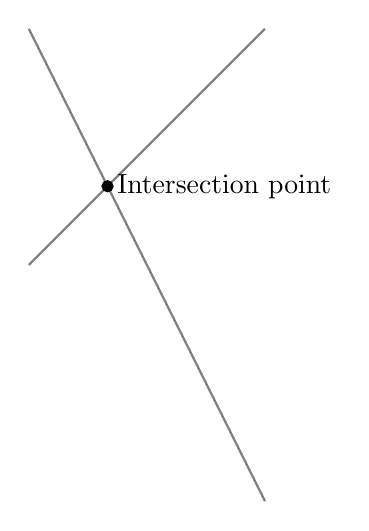
\begin{tikzpicture}
\draw[gray, thick] (-1,2) -- (2,-4);
\draw[gray, thick] (-1,-1) -- (2,2);
\filldraw[black] (0,0) circle (2pt) node[anchor=west] {Intersection point};
\end{tikzpicture}


\begin{tikzpicture}
\draw (-2,0) -- (2,0);
\filldraw [gray] (0,0) circle (2pt);
\draw (-2,-2) .. controls (0,0) .. (2,-2);
\draw (-2,2) .. controls (-1,0) and (1,0) .. (2,2);
\end{tikzpicture}

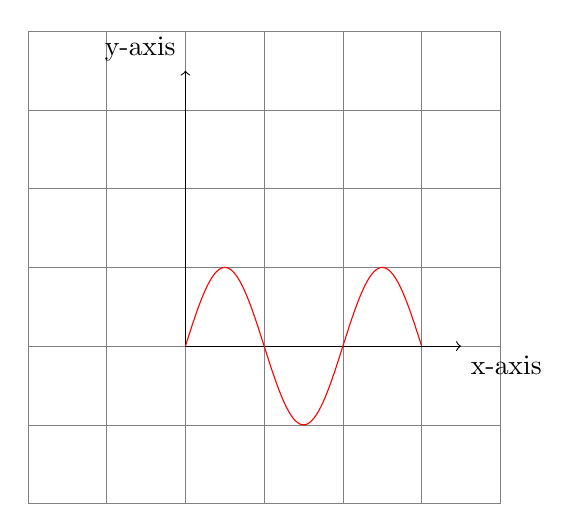
\begin{tikzpicture}
% grid
\draw [help lines] (-2,-2) grid (4,4);
% coordinate system
\draw[->] (0,0) -- (3.5,0) node[anchor=north west] {x-axis};
\draw[->] (0,0) -- (0,3.5) node[anchor=south east] {y-axis};

% draw a sine curve. The trigonometric functions assume that x is in degrees; to express x in radians follow it with the notation "r"
\draw [red, domain=0:3, samples=100] plot (\x, {sin(pi*\x r)});

\end{tikzpicture}

% Bloch sphere
\begin{tikzpicture}[scale=1.5]

  % Define radius and spherical angles
  \def\r{2}
  \def\phi{-35}
  \def\theta{25}

  % Sphere
  \draw (0,0) circle (\r); % circle
  \draw[thick,dashed] (0,0) ellipse (\r{} and \r/3); % ellipse

  % Bloch vector
  %\node (orig) at (0,0)          [] {};
  %\node (a)    at (\r/3,2*\r/3)  [] {};
  %\node (b)    at (\r/3,-\r/5)   [] {};
  %\node [above] at (\r/3,2*\r/3) {$s\le 3$};

  %\draw[] (orig) -- (a) -- (b) -- (orig);
  %\draw (0,0) -- (\r/3,2*\r/3) -- (\r/3,-\r/5) -- cycle [];
  \draw[dashed,red,thick] (0,0) -- ({1*\r*cos(\phi)*sin(\theta)},{1*\r*sin(\phi)*sin(\theta)}) -- ++(0,{\r*cos(\theta)});

  \draw[] (0,0)

  %\draw[] (0,0) -- (60:3*\r/4);
  %\draw[thick,dashed] (60:3*\r/4) -- ++(0,-3*\r/4) -- (0,0);


  % ANGLES
  \draw (0,0) arc [start angle=60, end angle=90, radius=\r/2];
  %\draw (3mm,3mm) arc [start angle=0, end angle=30, radius=3mm];

  %\draw (-\r/5,-\r/3) arc [start angle=-120, end angle=-30, radius=4mm];

  %\draw (0,0) node[] (orig) {} -- (\r/3,2*\r/3)
  %            node[circle,fill,inner sep=1,label=above:$|\psi\rangle$] (a) {};
  %\draw[dashed] (orig) -- (\r/3,-\r/5) node (phi) {} -- (a);

  % Coordinate system
  \draw[->] (0,0) -- (-135:\r)           node[below] (x1) {$\hat{\mathbf{x}}$};
  \draw[->] (0,0) -- (\r,0)            node[right] (x2) {$\hat{\mathbf{y}}$};
  \draw[->] (0,0) -- (0,\r)            node[above] (x3) {$\hat{\mathbf{z}}$};

  % Angles
  %\pic [draw,angle radius=.5cm,"$\phi$"] {angle = x1--orig--phi};
  %\pic [draw,angle radius=.8cm,"$\theta$"] {angle = a--orig--x3};

  % Computational basis states
  \filldraw[fill=white] (0,2)   circle (2pt) node[anchor=south west] {$|0\rangle$};
  \filldraw[fill=white] (0,-2)  circle (2pt) node[anchor=north west] {$|1\rangle$};

\end{tikzpicture}

% Make a circle with a coordiante system, grid lines, sine and cosine, that shows
% pythagoras

\end{document}
